
\chapter{概形的一些性质}
\label{ch:properties-of-schemes}

既然已经定义了\trScheme{}这个概念，我们就可以定义\trScheme{}的一些有用性质了。每见到一条定义，都应当在你自选的具体例子上把它试用一番，比如你最钟爱的那些形如 $\Spec\mathbb{C}[x_1,\dots,x_n]/(f_1,\dots,f_r)$ 的\trScheme。


\section{拓扑性质}

\trConnected、\trConnectedComponent、（不）可约、\trIrreducibleComponent、\trQuasicompact、\trGenerization、\trSpecialization、\trGenericPoint、\trNoetherian{}\trTopologicalSpace{}与\trClosedPoint{}的定义都已在 \S3.6 中给出。你脑中应当为其中每一个观念都备有图像。

\cref{ex:integral-domain-irreducible} 已表明 $\mathbb{A}^n_k$ 是\trIrreducible{}的（这很容易）。这个论证「在粘合之下表现良好」，由此得到：

\textbf{5.1.A.（容易的练习）}\quad 证明：$\mathbb{P}^n_k$ 是\trIrreducible{}的。

\textbf{5.1.B.（练习）}\quad 练习~3.7.F 已证明：对\trAffineScheme，诸\trIrreducible{}闭子集与诸点之间存在双射（把点 $p$ 送到闭子集 $\overline{\{p\}}$ 的映射是双射）。证明：对一般的\trScheme{}这件事也成立。

\textbf{5.1.C.（容易的练习）}\quad 证明：若概形 $X$ 拥有有限\trCover{} $X=\bigcup_{i=1}^{n}\Spec A_i$（其中诸 $A_i$ 皆\trNoetherian），则 $X$ 是\trNoetherian{}\trTopologicalSpace（\S3.6.14）。（我们很快就会把带有这种\trCover{}的概形称作\emph{\trNoetherian{}概形}，\S5.3.4。）提示：证明一个作为\trNoetherian{}子空间之有限并的\trTopologicalSpace{}自身也是\trNoetherian{}的。

于是 $\mathbb{P}^n_k$ 与 $\mathbb{P}^n_{\mathbb{Z}}$ 都是\trNoetherian{}\trTopologicalSpace：我们是用有限多个\trNoetherian{}环的谱粘合起来造出它们的。

\textbf{5.1.D.（容易的练习）}\quad 证明：概形 $X$ 是\trQuasicompact{}的，当且仅当它能写成有限多个\trAffine\trOpenSubscheme{}之并。（于是对任意\trRing{} $A$，$\mathbb{P}^n_A$ 都\trQuasicompact。）

\textbf{5.1.E.（练习：\trQuasicompact{}概形有\trClosedPoint）}\quad 证明：若 $X$ 是\trQuasicompact{}概形，则每个点的闭包中都含有一个\trClosedPoint。证明：$X$ 的每个非空\trClosedSubset{}都含有 $X$ 的一个\trClosedPoint。特别地，每个非空\trQuasicompact{}概形都有\trClosedPoint。（警告：确有不含任何\trClosedPoint{}的非空概形——例如练习~15.2.P——所以你的论证最好当真用到\trQuasicompactness{}假设！）

这条练习日后常按如下方式使用。设概形的点有某条性质 $P$，且这条性质是「开」的（若点 $p$ 具有性质 $P$，则存在 $p$ 的某个开\trNeighborhood{} $U$，使 $U$ 中所有的点都具有性质 $P$），那么要检验一个\trQuasicompact{}概形是否\emph{所有}的点都具有性质 $P$，只需检验诸\trClosedPoint{}即可。（这一哲学的第一个例子是练习~5.2.E。）这在概形与\trVariety{}的经典理论之间建立了联系——传统\trVariety{}的点正是相应概形的\emph{闭}点（本质上靠的是\trNullstellensatz；参看 \S3.6.9 与练习~5.3.F）。在许多好的情形，\trClosedPoint{}是\trDense{}的（比如对\trVariety{}正是如此；再参看 \S3.6.9 与练习~5.3.F），但在一些基本情形中并非如此（参看\cref{ex:closed-points-dense}(b)）。

\textbf{5.1.1.\ \trQuasiSeparated{}概形。}\quad \trQuasiseparatedness{}是个古怪的观念，但对某些人来说正巧派得上用场。（警告：日后我们会发觉，这其实是\emph{\trMorphism}的性质而非概形的性质，\S8.3.1。）不过大多数人可以对这个观念置之不理，因为他们在现实生活中会遇到的概形全都具有这条性质。称一个\trTopologicalSpace{}是\textbf{\trQuasiSeparated}（quasiseparated）的，若任何两个\trQuasicompact{}\trOpenSubset{}的交仍是\trQuasicompact{}的。（名称中「分离性」的动机在于：它是\emph{\trSeparated}（separated）的弱化版本——对后者，任何两个\emph{\trAffine}开集之交都是\trAffine{}的；参看命题~11.2.13。）

\textbf{5.1.F.（短练习）}\quad 证明：概形是\trQuasiSeparated{}的，当且仅当任何两个\trAffine\trOpenSubscheme{}的交都是有限多个\trAffine\trOpenSubscheme{}之并。

\textbf{5.1.G.（练习）}\quad 证明\trAffineScheme{}都是\trQuasiSeparated{}的。（可能的提示：练习~5.1.F。）

\textbf{5.1.H.（练习）}\quad 证明：概形 $X$ 是\trQuasiSeparated{}的，当且仅当\emph{存在} $X$ 的一个由\trAffine\trOpenSubscheme{}构成的\trCover，其中任何两个之交也被\emph{有限}多个\trAffine\trOpenSubscheme{}覆盖。

我们将会看到，\trQuasiseparatedness{}在定理中（与\trQuasicompactness{}相配合）将是一条有用的假设，而且各种有趣的概形——仿射、局部诺特与分离（分别见练习~5.1.G、练习~5.3.A 与练习~11.2.D）——都是\trQuasiSeparated{}的；这将使我们能把定理陈述得更简洁（例如说「若 $X$ \trQuasicompact{}且\trQuasiSeparated」，而不必说「若 $X$ \trQuasicompact，且这条、那条或另外某条性质成立」）。

「\trQuasicompact{}且\trQuasiSeparated」意味着某件具体的事：

\textbf{5.1.I.（练习）}\quad 证明：概形 $X$ \trQuasicompact{}且\trQuasiSeparated{}，当且仅当 $X$ 能被有限多个\trAffine\trOpenSubscheme{}覆盖，其中任何两个之交也被有限多个\trAffine\trOpenSubscheme{}覆盖。

\textbf{5.1.2.}\ \emph{Qcqs。}\quad 当你在一条定理的假设中见到「\trQuasicompact{}且\trQuasiSeparated」时，应当把这当作一个提示：你将会用到上述解读，而且有限性将以本质的方式被用到。这组假设实在太过常见，以致人们常把它简称为 \textbf{qcqs}（例如见 Qcqs 引理~6.2.9）。

\textbf{5.1.J.（容易的练习）}\quad 证明：一切射影 $A$-\trScheme{}都既\trQuasicompact{}又\trQuasiSeparated。（提示：利用定义中的\trGradedRing{}为\trFinitelyGenerated{}这一事实——那有限个\trGenerator{}会把你引向一组覆盖。）

\textbf{5.1.K.（练习：一个非\trQuasiSeparated{}概形）}\quad 设 $X=\Spec k[x_1,x_2,\dots]$，并令 $U$ 为 $X\setminus[\mathfrak{m}]$，其中 $\mathfrak{m}$ 是\trMaximalIdeal{} $(x_1,x_2,\dots)$。取 $X$ 的两份拷贝，沿 $U$ 粘合起来（「原点加倍了的仿射 $\infty$-空间」；「有限维」版本见例~4.4.5 与\cref{ex:doubled-origin-plane}）。证明：所得的概形不\trQuasiSeparated。提示：这个「\trOpenEmbedding」$U\subset X$ 早在\cref{ex:spec-quasicompact}(b) 中就出现过，是\trAffineScheme{}的非\trQuasicompact{}\trOpenSubset{}的一个例子。

\textbf{5.1.3.}\ \emph{\trDimension{}。}\quad 有一个非常重要的拓扑观念是\emph{\trDimension}。（令人惊叹的是，这竟是一个\emph{拓扑}层面的想法。）不过它虽然在直观上十分基本，却更为困难，所以我们把它推迟到第~12~章。


\section{\trReducedness{}与\trIntegrality{}}

回想一下，概形令人警觉的事情之一便是：函数并不由其在各点处的值决定，而这正是%
\trNilpotent{}元在作祟（\S3.2.12）。

\textbf{5.2.1.}\ \emph{\trhDefinition{}。}\quad 我们称一个\trScheme{} $X$ 是%
\textbf{\trReduced}（reduced）的，如果它的诸\trStalk{} $\OO_{X,p}$ 都没有非零%
\trNilpotent{}元（对一切 $p$）。\trReducedness{}按定义就是一条\trStalkLocal{}性质（\S2.4.1）。

\textbf{5.2.A.（练习）}\quad 证明：若 $f$ 与 $g$ 是\trReduced{}\trScheme{}上的两个函数（即 $\OO_X$ 的两个%
\trGlobalSections），二者在所有点处取值都相同，则 $f=g$。（两条提示：单射%
$\OO_X(\mathsf{U})\hookrightarrow\prod_{p\in\mathsf{U}}\OO_{X,p}$，来自%
\cref{ex:sections-determined-by-germs}；以及\trNilradical{}是全体\trPrimeIdeal{}的交，
来自\cref{thm:nilradical-intersection-primes}。）

\textbf{5.2.B.（练习）}\quad 回想：若一个\trRing{}没有非零\trNilpotent{}元，就称它是\emph{\trReduced}的（\S3.2.14）。
证明：$A$ 是\trReduced{}环，当且仅当 $\Spec A$ 是\trReduced{}的。再证明：若对 $X$ 的
每个\trOpenSet{} $\mathsf{U}$，$\OO_X(\mathsf{U})$ 都是\trReduced{}环，则\trScheme{}
$X$ 是\trReduced{}的。

\textbf{5.2.C.（容易的练习）}\quad 证明 $\mathbb{A}^n_k$ 与 $\mathbb{P}^n_k$ 都是\trReduced{}的。

\trScheme{} $\Spec k[x,y]/(y^2,xy)$ 是非\trReduced{}的。在图~\ref{fig:nonreduced-y2xy}
中勾画它时，我们曾示意：那团\trFuzz{}标示出的正是原点处的非\trReducedness{}。下面的
练习便是把这件事说精确的第一次尝试。

\textbf{5.2.D.（练习）}\quad 证明 $\bigl(k[x,y]/(y^2,xy)\bigr)_x$ 没有非零\trNilpotent{}元。（可能的提示：借助几何
图画，证明它\trIsomorphic{}于另一个\trRing。\cref{ex:xy-localization-isomorphism} 也许
能给出另一条提示。）再证明：$\Spec k[x,y]/(y^2,xy)$ 中唯一具有非\trReduced{}\trStalk{}
的点就是原点。

\textbf{5.2.E.（不重要的练习）}\quad 设 $X$ 是\trQuasicompact{}\trScheme，证明：只需在\trClosedPoint{}处检验\trReducedness{}。提示：
别试图证明\trReducedness{}是一条\textbf{开条件}（open condition，见注记~5.2.2）。作为替代，利用
练习~5.1.E 证明：任何非\trReduced{}的点，其闭包中都有一个非\trReduced{}的%
\trClosedPoint。（这个结果很有意思，但我们用不上它。）

\textbf{5.2.2.}\ \emph{\trhRemark{}。}\quad 我们将在练习~6.6.N 中看到：对%
\trLocally\trNoetherian{}\trScheme，\trReducedness{}是一条开条件。但一般地，\trReducedness{}并不是开条件。
你或许能把
\[
X=\Spec\mathbb{C}[x,y_1,y_2,\dots]\big/\bigl(y_1^2,\,y_2^2,\,y_3^2,\,\dots,\,(x-1)y_1,\,(x-2)y_2,\,(x-3)y_3,\,\cdots\bigr)
\]
的底\trTopologicalSpace{}与 $\Spec\mathbb{C}[x]$ 的底\trTopologicalSpace{}认同起来，
进而证明：$X$ 的非\trReduced{}点恰是与正整数相对应的那些\trClosedPoint。此集合的%
\trComplement{}不是\trZariski{}开集。

\textbf{5.2.3.}\ \hard\ \emph{给专家的\trhWarning{}。}\quad 若\trScheme{} $X$ 是%
\trReduced{}的，则（据练习~5.2.B）其\trGlobalSections{}所成之%
\trRing{}是\trReduced{}的。然而逆命题不真。你现在已经有足够的知识来验证：若 $X$ 是
$\mathbb{P}^2_k$ 中由 $x^2=0$ 割出的\trScheme，则 $\Gamma(X,\OO_X)\cong k$，而 $X$ 非%
\trReduced{}。（这个例子日后还将在 \S11.4.7 与 \S18.6.U 中出现。）

\textbf{5.2.F.（练习）}\quad 设 $X$ 是\trQuasicompact{}的，而 $f$ 是一个在 $X$ 的所有点处都消失的函数。证明：存在
某个 $n$ 使得 $f^n=0$。再证明：当 $X$ 不\trQuasicompact{}时，这可能失效。（本练习较不
重要，但它说明了我们为何钟爱\trQuasicompactness，并给出了\trQuasicompactness{}不成立
时的一种标准病态。）提示：取诸 $\Spec A_n$ 的一个无穷\trDisjointUnion，其中%
$A_n:=k[\epsilon]/(\epsilon^n)$。这个\trScheme{}日后还将在 \S9.4.2（其图画见图~9.5）
以及警示/例~9.4.11 中再次出现。

\textbf{5.2.4.}\ \emph{\trhDefinition{}。}\quad \trScheme{} $X$ 称为%
\textbf{\trIntegral}（integral）的，如果它非空，并且对 $X$ 的每个非空\trOpenSubset{}%
$\mathsf{U}$，$\OO_X(\mathsf{U})$ 都是\trIntegralDomain。

\textbf{5.2.G.（重要练习）}\quad 证明：\trScheme{} $X$ 是\trIntegral{}的，当且仅当它既\trIrreducible{}又\trReduced{}。
（于是我们把\trIntegral{}\trScheme{}画成：「一整块，不惹\trFuzz{}。」可能的提示：%
\cref{ex:vanishing-locus-closed}。）

\textbf{5.2.H.（练习）}\quad 证明：\trAffineScheme{} $\Spec A$ 是\trIntegral{}的，当且仅当 $A$ 是\trIntegralDomain。

\textbf{5.2.I.（练习）}\quad 设 $X$ 是\trIntegral{}\trScheme。则 $X$（因为它\trIrreducible）有一个\trGenericPoint{}%
$\eta$。设 $\Spec A$ 是 $X$ 的任一非空\trAffine\trOpenSubset。证明：$\OO_{X,\eta}$%
（即 $\OO_X$ 在 $\eta$ 处的\trStalk）被自然地认同于 $A$ 的\trFractionField{}%
$\mathrm{K}(A)$。它称为 $X$ 的\textbf{\trFunctionField}（function field）$\mathrm{K}(X)$。
在 $X$ 的任何非空\trOpenSet{}上都能把它算出来，因为任何这样的\trOpenSet{}都含有%
\trGenericPoint。$\mathrm{K}(X)$ 的元素称为 $X$ 上的\textbf{\trRationalFunction}
（rational function；日后将在定义~6.6.36 中进一步推广）。

\textbf{5.2.J.（练习）}\quad 设 $X$ 是\trIntegral{}\trScheme。证明：只要 $\mathsf{V}\neq\varnothing$，诸%
\trRestrictionMap{} $\operatorname{res}_{\mathsf{U},\mathsf{V}}\colon\OO_X(\mathsf{U})
\to\OO_X(\mathsf{V})$ 就都是包含。设 $\Spec A$ 是 $X$ 的任一非空\trAffine\trOpenSubset%
（于是 $A$ 是\trIntegralDomain）。证明：自然映射
$\OO_X(\mathsf{U})\to\OO_{X,\eta}=\mathrm{K}(A)$（其中 $\mathsf{U}$ 是任一非空%
\trOpenSubset，而 $\eta$ 是\trGenericPoint）是包含。

于是，不可约\trVariety（日后定义的\trIntegral{}\trScheme{}的一个重要例子）便享有一件
方便的性质：不同\trOpenSet{}上的\trSection{}可以被看作同一个\trRing{}的子集。特别地，
\trRestrictionMap（除指向空集的情形外）总是包含，而粘合也变得容易：$\mathsf{U}$ 的一个%
\trCover{} $\mathsf{U}_i$ 上的诸函数 $f_i$（$i$ 跑遍一个\trIndexSet）能够粘合，当且仅当
它们是 $\mathrm{K}(X)$ 的同一个元素。这是（不可约的）\trVariety{}通常先于\trScheme{}被
引入的原因之一。

\textbf{5.2.5.}\ \emph{\trhCaveat{}。}\quad \trIntegrality{}不是\trStalkLocal{}性质（两个%
\trIntegral{}\trScheme{}的\trDisjointUnion{}不是\trIntegral{}的，因为据%
\cref{ex:product-ring-homeomorphism}，$\Spec A\sqcup\Spec B=\Spec(A\times B)$），但它
差一点就是；见练习~5.3.C。


\section{仿射通信引理与可\trAffineLocal{}检验的性质}

本节意在处理概形定义中某个棘手之处。我们已把概形定义为一个\trTopologicalSpace{}连同其上的一个环层，且它能被诸\trAffineScheme{}覆盖。于是，覆盖中的仿射开集我们全都有了，却不知道该如何让其中任意两个互通消息。说得再直白些：若我有一个仿射覆盖，你也有一个仿射覆盖，我们想把二者加以比较，而我在自己的覆盖上算出了某个东西，那么总该有办法让我们凑到一起，弄清怎样把我的计算翻译到你的覆盖上去。\trAffineCommunicationLemma{}~5.3.2 将为此提供一台方便的机器。

托这条引理之福，我们能定义一大批概形的重要性质。这些性质都是「\trAffineLocal{}」（affine-local）的，意即它们可以在任何一个仿射覆盖——也就是由仿射开集构成的覆盖——上加以检验。（待\trAffineCommunicationLemma{}陈述过后，我们会把这一点表述得更正式。）我们喜欢这类性质，因为随我们喜欢用哪个仿射覆盖来检验都行。若所论的概形\trQuasicompact，则只需检验有限多个仿射开集。

\textbf{5.3.1.\ \trhProposition{}。}\ ——\ \emph{设 $\Spec A$ 与 $\Spec B$ 是概形 $X$ 的两个\trAffine\trOpenSubscheme。则 $\Spec A\cap\Spec B$ 是一族开集之并，其中每个开集都同时是 $\Spec A$ 与 $\Spec B$ 的\trDistinguishedOpen\trSubscheme{}。}

\begin{figure}[htbp]
  \centering
  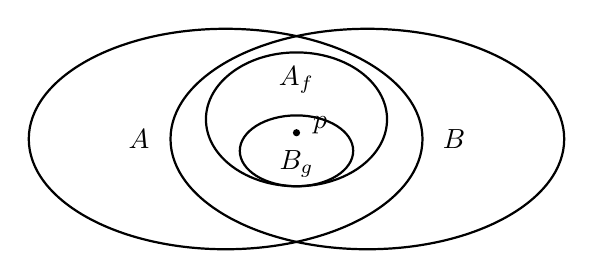
\begin{tikzpicture}[scale=1.0,line width=0.8pt]
    \draw (-0.9,0) ellipse (2.5 and 1.4);
    \draw (0.9,0) ellipse (2.5 and 1.4);
    \node at (-2.0,0) {$\Spec A$};
    \node at (2.0,0) {$\Spec B$};
    \draw (0,0.25) ellipse (1.15 and 0.85);
    \node at (0,0.75) {$\Spec A_f$};
    \draw (0,-0.15) ellipse (0.72 and 0.45);
    \node at (0,-0.32) {$\Spec B_g$};
    \fill (0,0.08) circle (1.3pt);
    \node at (0.30,0.18) {$p$};
  \end{tikzpicture}
  \caption{一个展示「两个仿射开集的交可以被在两个仿射开集中同时特异的开集覆盖」的小技巧。（依原书手绘图重绘。）}\label{fig:affine-communication-trick}
\end{figure}

\emph{证明。}\ （见图~\ref{fig:affine-communication-trick}）任取一点 $p\in\Spec A\cap\Spec B$，我们在 $\Spec A\cap\Spec B$ 中构造 $p$ 的一个开\trNeighborhood，使它同时在 $\Spec A$ 与 $\Spec B$ 中都特异。取 $\Spec A$ 的一个含于 $\Spec A\cap\Spec B$ 且包含 $p$ 的\trDistinguishedOpen{} $\Spec A_f$；再取 $\Spec B$ 的一个含于 $\Spec A_f$ 且包含 $p$ 的\trDistinguishedOpen{} $\Spec B_g$。于是 $g\in\Gamma(\Spec B,\OO_X)$ 限制为一个元素 $g'\in\Gamma(\Spec A_f,\OO_X)=A_f$。$g$ 与 $g'$ 在 $\Spec A_f$ 上消失的点相同，故
\[
\Spec B_g=\Spec A_f\setminus\{[p]\ :\ g'\in p\}=\Spec\bigl(A_f\bigr)_{g'}.
\]
若 $g'=g''/f^n$（其中 $g''\in A$），则 $\Spec(A_f)_{g'}=\Spec A_{fg''}$，证明便告完成。\hfill$\square$

下面这条容易的结果对我们至关重要。

\textbf{5.3.2.\ \trAffineCommunicationLemma。}\ ——\ \emph{设 $P$ 是概形 $X$ 的一些\trAffine\trOpenSubscheme{}所享有的某条性质，使得对 $X$ 的任何\trAffine\trOpenSubscheme{} $\Spec A\hookrightarrow X$：}
\begin{enumerate}[label=(\roman*)]
  \item \emph{若 $\Spec A\hookrightarrow X$ 具有性质 $P$，则对任意 $f\in A$，$\Spec A_f\hookrightarrow X$ 也具有性质 $P$；}
  \item \emph{若 $(f_1,\dots,f_n)=A$（即诸 $\Spec A_{f_i}$ 覆盖 $\Spec A$；参看\cref{ex:distinguished-cover-unit-ideal}），且 $\Spec A_{f_i}\hookrightarrow X$ 对一切 $i$ 都具有 $P$，则 $\Spec A\hookrightarrow X$ 也如此。}
\end{enumerate}
\emph{再设 $X=\bigcup_{i\in I}\Spec A_i$，其中每个 $\Spec A_i$ 都具有性质 $P$。则 $X$ 的每个\trAffine\trOpenSubscheme{}也具有 $P$。}

满足 (i) 与 (ii) 的性质称为\textbf{\trAffineLocal{}}（affine-local）的。这个名称的一个动机是：凭借这条引理，要想判定\emph{每个}\trAffine\trOpenSubscheme{}是否具有该性质，只需在\emph{任何一个}仿射覆盖上检验即可。

举个例子：\trReducedness{}就是一条\trAffineLocal{}的性质。更一般地，任何\trStalkLocal{}的性质（概形具有性质 $P$，当且仅当它的所有\trStalk{}都具有性质 $Q$）必然是\trAffineLocal{}的（概形具有性质 $P$，当且仅当它的所有仿射开集都具有性质 $R$，而仿射概形具有性质 $R$，当且仅当它的所有\trStalk{}都具有性质 $Q$）。但 $Q$ 的正确定义有时并不那么显然；例如可参看下一节关于\trNormality{}的讨论。

\emph{证明。}\ 设 $\Spec A$ 是 $X$ 的一个仿射\trSubscheme{}。用有限多个\trDistinguishedOpen{} $\Spec A_{g_j}$ 覆盖 $\Spec A$，其中每个都在某个 $\Spec A_i$ 中特异。由命题~5.3.1 与 $\Spec A$ 的\trQuasicompactness{}（\cref{ex:spec-quasicompact}(a)），这样做是可行的。由 (i)，每个 $\Spec A_{g_j}$ 都具有 $P$。由 (ii)，$\Spec A$ 具有 $P$。\hfill$\square$

适当地选取性质 $P$，我们便定义出概形的一些重要性质。

\textbf{5.3.3.\ \trhProposition{}。}\ ——\ \emph{设 $A$ 是一个\trRing，且 $(f_1,\dots,f_n)=A$。}
\begin{enumerate}[label=(\alph*)]
  \item \emph{若 $A$ 是\trNoetherian{}环，则每个 $A_{f_i}$ 亦然。若每个 $A_{f_i}$ 都\trNoetherian，则 $A$ 亦然。}
  \item \emph{设 $B$ 是一个\trRing，而 $A$ 是一个 $B$-\trAlgebra（于是对一切 $g\in A$，$A_g$ 都是 $B$-\trAlgebra）。若 $A$ 是\trFinitelyGenerated{}的 $B$-\trAlgebra，则每个 $A_{f_i}$ 亦然。若每个 $A_{f_i}$ 都是\trFinitelyGenerated{}的 $B$-\trAlgebra，则 $A$ 亦然。}
\end{enumerate}

这些断言我们稍后便证（\S5.3.9）。但为了给你一个读证明的动力，我们先\emph{假定}命题~5.3.3 成立，由此给出一些有趣的定义与结果。

\textbf{5.3.4.}\ \emph{重要定义。}\quad 设 $X$ 是一个概形。若 $X$ 能被诸\trAffine\trOpenSet{} $\Spec A$ 覆盖，其中诸 $A$ 都\trNoetherian，就称 $X$ 是一个\textbf{\trLocally\trNoetherian{}\trScheme}（locally Noetherian scheme）。若此外 $X$ 还\trQuasicompact——等价地，能被有限多个这样的\trAffine\trOpenSet{}覆盖——就称 $X$ 是一个\textbf{\trNoetherian{}\trScheme}（Noetherian scheme）。（日后我们会见到许多形如「若 $X$ 具有此性质，就称它为局部 $Q$；若进而 $X$ 还\trQuasicompact，就称它是 $Q$」的定义。）由练习~5.1.C，\trNoetherian{}\trScheme{}的底\trTopologicalSpace{}是\trNoetherian{}的。于是由\cref{ex:noetherian-open-quasicompact}，\trNoetherian{}\trScheme{}的所有\trOpenSubset{}都\trQuasicompact。

\textbf{5.3.A.（练习）}\quad 证明：\trLocally\trNoetherian{}\trScheme{}都是\trQuasiSeparated{}的。

\textbf{5.3.B.（练习）}\quad 证明：\trNoetherian{}\trScheme{}只有有限多个\trIrreducibleComponent。（提示：命题~3.6.15。）证明：\trNoetherian{}\trScheme{}只有有限多个\trConnectedComponent，其中每一个都是有限多个\trIrreducibleComponent{}之并。

\textbf{5.3.C.（练习）}\quad 证明：\trNoetherian{}\trScheme{} $X$ 是\trIntegral{}的，当且仅当 $X$ 非空、\trConnected，且所有\trStalk{} $\OO_{X,p}$ 都是\trIntegralDomain。于是，在「好情形」下，\trIntegrality{}是局部条件（诸\trStalk{}为\trIntegralDomain）与整体条件（\trConnected）二者之并。提示：回想 \trIntegral{}＝\trIrreducible{}＋\trReduced（练习~5.2.G）。若一个概形的诸\trStalk{}都是\trIntegralDomain，则它是\trReduced{}的（\trReducedness{}是一条\trStalkLocal{}条件，定义~5.2.1）。若概形 $X$ 的底\trTopologicalSpace{}是\trNoetherian{}的，则 $X$ 只有有限多个\trIrreducibleComponent{}（由上一练习）；若其中两个在一点 $p$ 相交，则 $\OO_{X,p}$ 不是\trIntegralDomain。（把这件事从\trNoetherian{}\trScheme{}推广到\trLocally\trNoetherian{}\trScheme{}是轻而易举的：只须证明，一个\trConnected{}\trScheme{}是\trIrreducible{}的，当且仅当它非空，且具有一个由开\trIrreducible{}子集构成的\trCover。但某些\trNoetherian{}假设是必要的；参看 [Stacks, tag 0568]。）

\textbf{5.3.5.}\ \emph{不重要的警示。}\quad \trNoetherian{}\trScheme{}的\trGlobalSections{}环未必\trNoetherian；参看练习~19.11.H。

\textbf{5.3.6.\ 给定域 $k$ 之上、或更一般地给定环 $A$ 之上的概形（$A$-\trScheme）。}\quad 你也许特别想在某个特定的域——比如 $\mathbb{C}$ 或 $\mathbb{Q}$——之上工作，或者在诸如 $\mathbb{Z}$ 的环之上工作。受此驱动，我们定义\textbf{$A$-\trScheme}（$A$-scheme）或\textbf{$A$ 上的概形}（scheme over $A$）的概念，其中 $A$ 是一个\trRing：它是一个概形，其\trStructureSheaf{}（在一切\trOpenSet{}上）的诸\trSection{}环都是 $A$-\trAlgebra，并且所有\trRestrictionMap{}都是 $A$-\trAlgebra{}之间的映射。（正如早先诸如\trQuasiseparatedness{}那样的一些观念，这一观念日后将在练习~7.3.I 中被恰当地理解为一个「相对概念」；它的数据是一个\trMorphism{} $X\to\Spec A$。）现在设 $X$ 是一个 $A$-\trScheme。若 $X$ 能被诸\trAffine\trOpenSet{} $\Spec B_i$ 覆盖，且每个 $B_i$ 都是\trFinitelyGenerated{}的 $A$-\trAlgebra，就称 $X$ \textbf{在 $A$ 上\trLocally\trFiniteType}（locally of finite type over $A$），或称它是一个\textbf{\trLocally\trFiniteType{} $A$-\trScheme}（locally finite type $A$-scheme）。（无可否认这套术语颇为累赘；等我们在 \S8.3.9 认识了\trMorphism{}之后，它会更显自然。）若进而 $X$ 还\trQuasicompact，就称 $X$ \textbf{在 $A$ 上\trFiniteType}（finite type over $A$），或称它是一个\textbf{\trFiniteType{} $A$-\trScheme}（finite type $A$-scheme）。注意：在 $k$ 或 $\mathbb{Z}$ 上（或者的确，在任何\trNoetherian{}环上）\trLocally\trFiniteType{}的概形是\trLocally\trNoetherian{}的；类似地，在任何\trNoetherian{}环上\trFiniteType{}的概形是\trNoetherian{}的。作为我们关键的「几何」例子：(i) $\Spec\mathbb{C}[x_1,\dots,x_n]/I$ 是一个\trFiniteType{} $\mathbb{C}$-\trScheme；(ii) $\mathbb{P}^n_{\mathbb{C}}$ 是一个\trFiniteType{} $\mathbb{C}$-\trScheme。（域 $\mathbb{C}$ 可以换成任意\trRing{} $A$。）

\textbf{5.3.D.（练习）}

(a)~（\emph{\trQuasiprojective{}蕴含有限型}）设 $X$ 是一个\trQuasiprojective{} $A$-\trScheme{}（定义~4.5.10），证明 $X$ 在 $A$ 上\trFiniteType。若进而还假定 $A$ \trNoetherian，证明 $X$ 是\trNoetherian{}\trScheme，从而只有有限多个\trIrreducibleComponent。

(b)~设 $U$ 是某射影 $A$-\trScheme{}的一个\trOpenSubscheme。证明 $U$ 在 $A$ 上\trLocally\trFiniteType。若 $A$ \trNoetherian，证明 $U$ \trQuasicompact，从而在 $A$ 上\trQuasiprojective{}，进而由 (a) 在 $A$ 上\trFiniteType。证明当 $A$ 不\trNoetherian{}时这可以不成立。更好的：给出某射影 $A$-\trScheme{}的一个非\trQuasicompact{}\trOpenSubscheme{}的例子（此时 $A$ 必为非\trNoetherian{}的）。（提示：傻例子~4.5.12。）

\textbf{5.3.7.\ \trVariety。}\quad 现在我们来与\trVariety{}的经典语言建立联系。一个既约且在 $k$ 上\trFiniteType{}的\trAffineScheme{}称为一个\textbf{仿射簇}（affine variety (over $k$)），或一个\textbf{仿射 $k$-簇}（affine $k$-variety）。一个既约的（拟）射影 $k$-\trScheme{}是一个\textbf{（拟）射影簇}（(quasi)projective variety (over $k$)），或一个\textbf{（拟）射影 $k$-簇}（(quasi)projective $k$-variety）。（警告：在文献中，簇的定义有时还被额外要求该概形\trIrreducible，或要求 $k$ 是\trAlgClosed{}的。）

\textbf{5.3.E.（练习）}

(a)~证明：$\Spec k[x_1,\dots,x_n]/I$ 是仿射 $k$-簇，当且仅当 $I\subset k[x_1,\dots,x_n]$ 是\trRadicalIdeal。

(b)~设 $I\subset k[x_0,\dots,x_n]$ 是分次的\trRadicalIdeal。证明：$\Proj k[x_0,\dots,x_n]/I$ 是射影 $k$-簇。（警示：例子 $I=(x_0^2,x_0x_1,\dots,x_0x_n)$ 表明，$\Proj k[x_0,\dots,x_n]/I$ 可以是射影 $k$-簇，而 $I$ 却并非根理想。）

我们要到 \S11.2.9 才会在一般情形下定义\trVariety；届时需要先有\trSeparatedness{}的观念，以便排除诸如原点加倍了的仿射直线（例~4.4.5）之类的可憎之物。但本节中我们将要陈述的关于仿射 $k$-簇的许多论断，都会自动适用于更一般的 $k$-簇。

\textbf{5.3.F.（练习）}\quad 证明：\trLocally\trFiniteType{} $k$-\trScheme{}的一点是\trClosedPoint，当且仅当\trStructureSheaf{}在该点处的\trStalk{}的\trResidueField{}是 $k$ 的一个\trFiniteFieldExtension。证明：在\trLocally\trFiniteType{} $k$-\trScheme{}上，诸\trClosedPoint{}是\trDense{}的。提示：\S3.6.9。（警告：即便在相当合理的概形上，\trClosedPoint{}也未必\trDense；参看\cref{ex:closed-points-dense}(b)。）

\textbf{5.3.8.}\ \emph{\trhDefinition{}。}\quad \trLocally\trFiniteType{} $k$-\trScheme{}（例如 $k$ 上的一个\trVariety）中\trClosedPoint{} $p$ 的\textbf{\trClosedPoint{}的\trDegree{}}（degree of a closed point），指的是域扩张 $\kappa(p)/k$ 的\trDegree{}。例如在 $\mathbb{A}^1_k=\Spec k[t]$ 中，点 $[(p(t))]$（其中 $p(t)\in k[t]$ \trIrreducible）的\trDegree{}就是 $\deg p(t)$。若 $k$ 是\trAlgClosed{}的，则每个\trClosedPoint{}的\trDegree{}都是 $1$。

\textbf{5.3.9.}\ \emph{\trhProposition{}~5.3.3 的证明。}\quad 依照\trAffineCommunicationLemma{}~5.3.2 的陈述，我们把每个部分的证明都按 (i) 与 (ii) 分开处理。

\emph{\trhProposition{}~5.3.3(a) 的证明。}\ (i)~设 $\phi:A\to A_f$ 是\trLocalization{}映射。若 $I_1\subsetneq I_2\subsetneq I_3\subsetneq\cdots$ 是 $A_f$ 的\trIdeal{}的一条严格增链，则可以验证 $J_1\subsetneq J_2\subsetneq J_3\subsetneq\cdots$ 是 $A$ 的\trIdeal{}的一条严格增链，其中 $J_i=\phi^{-1}(I_i)$。（我们把 $J_i$ 想成 $I_i\cap A$，只不过一般而言 $A$ 未必\trInjectiveMap{}到 $A_{f_i}$ 中。）显然 $J_i$ 是 $A$ 的\trIdeal。若有 $x/f^n\in I_{i+1}\setminus I_i$，其中 $x\in A$，则 $x\in J_{i+1}$，且 $x\notin J_i$（否则 $x(1/f)^n$ 也将属于 $I_i$）。

(ii)~设 $I_1\subsetneq I_2\subsetneq I_3\subsetneq\cdots$ 是 $A$ 的\trIdeal{}的一条严格增链。则对每个 $1\le i\le n$，
\[
I_{i,1}\subset I_{i,2}\subset I_{i,3}\subset\cdots
\]
是 $A_{f_i}$ 中\trIdeal{}的一条增链，其中 $I_{i,j}=I_j\otimes_A A_{f_i}$。尚须证明：对每个 $j$，存在某个 $i$ 使 $I_{i,j}\subsetneq I_{i,j+1}$；届时结论即随之而来。

\textbf{5.3.G.（练习）}\quad 完成命题~5.3.3(a) 的证明。（提示：若 $M:=I_j/I_{j-1}\neq0$，则由 $M\hookrightarrow\prod_i M_{f_i}$（\eqref{eq:module-equalizer-sequence}），某个 $M_{f_i}$ 非零。）

\emph{\trhProposition{}~5.3.3(b) 的证明。}\ 部分 (i) 是显然的：若 $A$ 由 $r_1$、……、$r_n$ 在 $B$ 上生成，则 $A_f$ 由 $r_1$、……、$r_n$、$1/f$ 在 $B$ 上生成。

(ii)~思路如下。由于诸 $f_i$ 生成 $A$，我们可以写出 $1=\sum c_if_i$，其中 $c_i\in A$。我们有诸 $A_{f_i}$ 的生成元：$r_{ij}/f_i^{k_i}$，其中 $r_{ij}\in A$。我断言：$\{f_i\}_i\cup\{c_i\}\cup\{r_{ij}\}_{ij}$ 作为 $B$-代数生成 $A$。理由如下。任取 $r\in A$。在 $A_{f_i}$ 中，我们可以把 $r$ 写成关于诸 $r_{ij}$ 与 $f_i$ 的某个多项式除以 $f_i$ 的某次巨大的幂。于是「在每个 $A_{f_i}$ 中，我们都已按要求描述了 $r$」，只差这枚烦人的分母。现在沿用\cref{thm:sheaf-on-distinguished-base}证明中那类「\trPartitionOfUnity{}」式的论证，把所有这些拼成一个单一的表达式，杀掉分母。证明你造出的表达式在每个 $A_{f_i}$ 中仍与 $r$ 一致。于是它确实就是 $r$（依据\trStructureSheaf{}的\trIdentityAxiom）。

\textbf{5.3.H.（练习）}\quad 把这个论证精确化。

至此，命题~5.3.3 的证明便告完成。\hfill$\square$


\section{\trNormality{}与\trFactoriality{}}

\textbf{5.4.1.}\ \emph{\trNormality{}。}\quad 我们现在可以定义概形的一条性质了，它说的是概形「离\trSmooth{}不太远」，称为\textbf{\trNormality}（normality），日后会非常顺手。我们日后会见到「\trLocally\trNoetherian{}\trNormal{}\trScheme{}满足\trHartogs{}引理」这句话（就\trNoetherian{}\trNormal{}\trScheme{}而言，即\trAlgebraic\trHartogs{}引理~13.5.19）：在一个\trCodimension{}为 $2$ 的集合之外定义的函数，可以延拓到该集合之上。（我们在 \S4.4.2 中已见过此事的端倪。）由此，无\trPole{}的\trRationalFunction（定义见练习~5.2.I）处处有定义（\trPole{}正是某些\trCodimension{}为 $1$ 的集合，函数在那里没有定义）。要把这件事说精确，我们还需要\trDimension{}与\trPole{}的定义。至于「\trSmoothness」（确切地说，是「\trRegularity{}」（regularity））蕴含\trNormality{}这一事实，见 \S13.8.7 与 \S26.3.5。

回想：称一个\trIntegralDomain{} $A$ 是\textbf{\trIntegrallyClosed{}}（integrally closed）的，如果 $A[x]$ 中任何\trMonicPolynomial{}在 $\mathrm{K}(A)$ 中的零点都必定落在 $A$ 自身之内。基本的例子是 $\mathbb{Z}$（缘由见练习~5.4.F）。称一个\trScheme{} $X$ 是\textbf{\trNormal}（normal）的，如果它的所有\trStalk{} $\OO_{X,p}$ 都\trNormal，即都是\trIntegralDomain，并且在其\trFractionField{}中\trIntegrallyClosed{}。（于是按定义，\trNormality{}是一条\trStalkLocal{}性质。）由于\trReducedness{}是一条\trStalkLocal{}性质（定义~5.2.1），\trNormal{}\trScheme{}都是\trReduced{}的。（有人或许愿意说：若 $\Spec A$ \trNormal，就称环 $A$ 是一个\textbf{\trNormal{}环}（normal ring），这样便把「\trIntegralClosure{}」（integral closure）的观念扩充到了并非\trIntegralDomain{}的环上。）

\textbf{5.4.A.（练习）}\quad 证明：\trIntegrallyClosed{}\trIntegralDomain{}在\trLocalization{}之下表现良好：设 $A$ 是\trIntegrallyClosed{}\trIntegralDomain，$S$ 是不含 $0$ 的\trMultiplicativeSubset，证明 $S^{-1}A$ 是\trIntegrallyClosed{}\trIntegralDomain。（提示：设 $x^n+a_{n-1}x^{n-1}+\cdots+a_0=0$（其中诸 $a_i\in S^{-1}A$）在\trFractionField{}中有一个根。把它变成 $A[x]$ 中另一个同样在该\trFractionField{}中有根的方程。）

在概形的每一个点处逐一检验\trNormality{}可不是什么乐事。多亏了这条练习，我们知道：若 $A$ 是\trIntegrallyClosed{}\trIntegralDomain，则 $\Spec A$ \trNormal。此外，对\trQuasicompact{}的概形或域上\trLocally\trFiniteType{}的概形，\trNormality{}可以在\trClosedPoint{}处检验——这多亏了这条练习，再加上这样一个事实：对这类概形，任何点都是某个\trClosedPoint{}的\trGenerization（练习~5.1.E 与练习~5.3.F）。

\trNormal{}\trScheme{}都是\trIntegral{}的，这并不真。例如，两个\trNormal{}\trScheme{}的\trDisjointUnion{}仍\trNormal。于是 $\Spec k\sqcup\Spec k\cong\Spec(k\times k)\cong\Spec k[x]/(x(x-1))$ \trNormal，但其\trGlobalSections{}环却不是\trIntegralDomain。

\textbf{5.4.B.（练习）}\quad 证明：\trNoetherian{}\trScheme{} \trNormal，当且仅当它是有限多个\trIntegral{}\trNoetherian{}\trNormal{}\trScheme{}的\trDisjointUnion。（提示：练习~5.3.C。）

我们已经逼近交换代数中的一条有用结果，索性一口气把它走到底。

\textbf{5.4.2.\ \trhProposition{}。}\ ——\ \emph{若 $A$ 是一个\trIntegralDomain，则下列三条等价。}
\begin{enumerate}[label=(\roman*)]
  \item \emph{$A$ 是\trIntegrallyClosed{}的。}
  \item \emph{对一切\trPrimeIdeal{} $\mathfrak{p}\subset A$，$A_{\mathfrak{p}}$ 都\trIntegrallyClosed{}。}
  \item \emph{对一切\trMaximalIdeal{} $\mathfrak{m}\subset A$，$A_{\mathfrak{m}}$ 都\trIntegrallyClosed{}。}
\end{enumerate}

\emph{证明。}\ 练习~5.4.A 表明\trIntegralClosedness{}在\trLocalization{}之下保持，故 (i) 蕴含 (ii)。显然 (ii) 蕴含 (iii)。

尚须证明 (iii) 蕴含 (i)。这个论证要用到一个相当精巧的构造，我们日后还会再度用到它。设 $A$ 不\trIntegrallyClosed{}。我们来证明：存在某个 $\mathfrak{m}$ 使 $A_{\mathfrak{m}}$ 也不\trIntegrallyClosed{}。设
\begin{equation*}\tag{5.4.2.1}\label{eq:monic-polynomial-root-s}
x^n+a_{n-1}x^{n-1}+\cdots+a_0=0
\end{equation*}
（其中诸 $a_i\in A$）在 $\mathrm{K}(A)\setminus A$ 中有解 $s$。设 $I$ 为 $s$ 的\textbf{\trIdealOfDenominators{}}（ideal of denominators）：
\begin{equation*}\tag{5.4.2.2}\label{eq:ideal-of-denominators}
I:=\{r\in A\;:\;rs\in A\}.
\end{equation*}
（注意，$I$ 显然是 $A$ 的一个\trIdeal。）由于 $1\notin I$，故 $I\neq A$。于是存在包含 $I$ 的某个\trMaximalIdeal{} $\mathfrak{m}$。那么 $s\notin A_{\mathfrak{m}}$，于是把方程 \eqref{eq:monic-polynomial-root-s} 放到 $A_{\mathfrak{m}}[x]$ 中看，便知 $A_{\mathfrak{m}}$ 也不\trIntegrallyClosed{}，正如所望。\hfill$\square$

\textbf{5.4.C.（不重要的练习）}\quad 若 $A$ 是一个\trIntegralDomain，证明：$A=\bigcap_{\mathfrak{m}}A_{\mathfrak{m}}$，其中交跑遍 $A$ 的所有\trMaximalIdeal。（我们不会用到这条练习，但它能让你好好操练一下\trIdealOfDenominators{}。）

\textbf{5.4.D.（与\trIdealOfDenominators{}有关的不重要的练习）}\quad 出于使用\trUFD{}的经验，人们或许会天真地指望：\trIdealOfDenominators{}是\trPrincipalIdeal。事情并非如此。作为反例，考虑我们的新朋友 $A=k[w,x,y,z]/(wz-xy)$（我们与它初次相逢是在\cref{thm:quadric-cone-section-example}，日后我们会认出它就是\trQuadricSurface{}上的\trCone），并考虑元素 $w/y=x/z\in\mathrm{K}(A)$。证明：$\mathrm{K}(A)$ 的这个元素的\trIdealOfDenominators{}是 $(y,z)$。

我们将会看到，上面这条练习中的 $I$ 不是\trPrincipalIdeal（练习~13.1.D——利用 $I$ 是某个\trGradedRing{}的\trHomogeneous\trIdeal{}这一事实，你或许能直接证明它）。但我们也会看到：在好的情形（\trNoetherian、\trNormal）下，\trIdealOfDenominators{}是「纯\trCodimension{} $1$」的——这正是\trAlgebraic\trHartogs{}引理~13.5.19 的内容。在该引理的证明（\S13.5.21）中，我们将给出\trIdealOfDenominators{}的一个几何解释。

\textbf{5.4.3.}\ \emph{\trFactoriality{}。}\quad 若\trScheme{} $X$ 的所有\trStalk{}都是\trUFD，就称 $X$ 是\textbf{\trFactorial{}的}（factorial）。（不重要的注记：\trAlgClosedField{}上的\trAffine\trVariety{}中，\trFactorial{}的点所成的\trLocus{}是一个\trOpenSubset，[BGS, p.~1]。）

\textbf{5.4.E.（练习）}\quad 证明：\trUFD{}的任何非零\trLocalization{}都是\trUFD。

\textbf{5.4.4.}\quad 于是，若 $A$ 是\trUFD，则 $\Spec A$ 唯一分解。逆命题不必成立；见练习~5.4.N。事实上我们将会看到：\textbf{\trEllipticCurve{}}（elliptic curve）是\trFactorial{}的，却\emph{没有}一个仿射开集是某个\trUFD{}的 $\Spec$（\S19.11.1）。因此，人们可以通过找出一个恰当的仿射\trCover{}来证明\trFactoriality{}，但\trFactorial{}的概形却未必\emph{存在}这样的\trCover。（有人或许会合情合理地把使 $\Spec A$ \trFactorial{}的环 $A$ 称为\textbf{\trFactorial{}环}（factorial ring）；这是比\trUFD{}严格更弱的观念。我们用不到这个术语。）

\textbf{5.4.5.}\ \emph{\trhRemark{}：如何检验一个环是否为\trUFD。}\quad 要检验一个\trNoetherian{}\trIntegralDomain{}是否为\trUFD，手段寥寥无几。一些有用的手段有：(0) 初等手段：带有\trEuclid{}算法的环，如 $\mathbb{Z}$、$k[t]$ 与 $\mathbb{Z}[i]$；\trUFD{}上的\trPolynomialRing{}——依据\trGauss{}引理（Gauss's Lemma，譬如见 [Lan, IV.2.3]）；(1) \trUFD{}的\trLocalization{}也是\trUFD（练习~5.4.E）；(2) \trHeight{}为 $1$ 的诸\trPrimeIdeal{}是\trPrincipalIdeal（命题~12.3.7）；(3) \trNormal{}且 $\mathrm{Cl}=0$（练习~15.5.P）；(4) \trNagata{}引理（Nagata's Lemma，练习~15.5.Q）。（警示：即便 $A$ 是\trUFD，$A[[t]]$ 也未必是；见 [Mat2, p.~165]。第一个例子由 P.~Salmon 给出：$A=k(u)[[x,y,z]]/(z^2+x^3+uz^6)$；见 [Sa, Dan]。）

\textbf{5.4.6.}\ \emph{\trFactoriality{}蕴含\trNormality{}。}\quad 我们喜欢\trFactoriality{}的一个理由是：它蕴含\trNormality。

\textbf{5.4.F.（重要练习）}\quad 证明：\trUFD{}都是\trIntegrallyClosed{}的。于是，\trFactorial{}的概形都\trNormal；而且若 $A$ 是\trUFD，则 $\Spec A$ \trNormal。（然而，环可以\trIntegrallyClosed{}而并非\trUFD——我们将在练习~5.4.L 中见到这一点。练习~5.4.N 不加证明地给出了另一个例子；在那个例子中，该环的 $\Spec$ 是\trFactorial{}的。把练习~5.4.L 稍加变通便会表明：概形可以\trNormal{}而不唯一分解；见练习~13.1.E。）

\textbf{5.4.7.}\ \emph{例子。}

\textbf{5.4.G.（容易的练习）}\quad 证明：下列概形都\trNormal：$\mathbb{A}^n_k$、$\mathbb{P}^n_k$、$\Spec\mathbb{Z}$。（照例，$k$ 是一个\trField。尽管「若 $A$ \trIntegrallyClosed{}，则 $A[x]$ 亦然」确实为真——见 [Bo, Ch.~5, \S1, no.~3, Cor.~2] 或 [E, Ex.~4.18]——但这并不是一个容易的事实，所以请不要在此使用它。）

\textbf{5.4.H.（称手的练习：日后给出许多富有启发的例子）}\quad 设 $A$ 是一个\trUFD{}且 $2$\trInvertible，并设 $z^2-f$ 在 $A[z]$ 中\trIrreducible。
\begin{enumerate}[label=(\alph*)]
  \item 证明：若 $f\in A$ 没有重复的素因子，则 $\Spec A[z]/(z^2-f)$ \trNormal。提示：$B:=A[z]/(z^2-f)$ 是一个\trIntegralDomain，因为 $(z^2-f)$ 在 $A[z]$ 中是\trPrimeIdeal。设有首一的 $F(T)\in B[T]$，使 $F(T)=0$ 在 $\mathrm{K}(B)\setminus\mathrm{K}(A)$ 中有解 $\alpha$。于是以 $\overline{F}(T)F(T)$ 代替 $F(T)$ 之后，不妨设 $F(T)\in A[T]$。又，$\alpha=g+hz$，其中 $g$、$h\in\mathrm{K}(A)$。此时 $\alpha$ 是 $Q(T)=0$ 的解，其中 $Q(T)=T^2-2gT+(g^2-h^2f)$ 是 $\mathrm{K}(A)[T]$ 中的\trMonicPolynomial{}，故可在 $\mathrm{K}(A)[T]$ 中分解 $F(T)=P(T)Q(T)$。由\trGauss{}引理，$2g$、$g^2-h^2f\in A$。设 $g=r/2$，$h=s/t$（$s$ 与 $t$ 无公因子，$r$、$s$、$t\in A$）。则 $g^2-h^2f=(r^2t^2-4s^2f)/4t^2$。于是 $t$\trInvertible。
  \item 证明：若 $f\in A$ 有重复的素因子，则 $\Spec A[z]/(z^2-f)$ 不\trNormal。
\end{enumerate}

\textbf{5.4.I.（练习）}\quad 证明：下列概形都\trNormal：
\begin{enumerate}[label=(\alph*)]
  \item $\Spec\mathbb{Z}[x]/(x^2-n)$，其中 $n$ 是模 $4$ 余 $3$ 的\trSquareFree{}（square-free）整数。警示：练习~5.4.H 的假设在此不适用，所以你只好直接来证。（你的论证或许也能顺带给出把 $3$ 换成 $2$ 时的结果。一个类似的论证表明：若 $n\equiv 1\pmod{4}$ 是\trSquareFree{}整数，则 $\mathbb{Z}[(1+\sqrt{n})/2]$ \trIntegrallyClosed{}。）
  \item $\Spec k[x_1,\dots,x_n]/(x_1^2+x_2^2+\cdots+x_m^2)$，其中 $\operatorname{char}k\neq 2$，$n\ge m\ge 3$。
  \item $\Spec k[w,x,y,z]/(wz-xy)$，其中 $\operatorname{char}k\neq 2$。这就是我们那个\trQuadricSurface{}上的\trCone{}的例子，来自\cref{thm:quadric-cone-section-example}与练习~5.4.D。提示：练习~5.4.J 也许用得上。（结论对 $\operatorname{char}k=2$ 同样成立，但不必为此费心。）
\end{enumerate}

\textbf{5.4.J.（练习：\trDiagonalize{}\trQuadraticForm{}）}\quad 设 $k$ 是一个\trCharacteristic{}不为 $2$ 的\trAlgClosedField。（$k$ \trAlgClosed{}这一假设并不必要，所以尽管去处理这个更一般的情形。此时 (a) 应稍作改写：「至多 $n$ 个平方数之和」应改为「至多 $n$ 个平方的 $k$-线性组合」。）
\begin{enumerate}[label=(\alph*)]
  \item 证明：$n$ 个变量的任何\textbf{\trQuadraticForm{}}（quadratic form）都能通过更换坐标「\trDiagonalize{}」为至多 $n$ 个平方数之和（例如 $uw-v^2=\bigl((u+w)/2\bigr)^2+\bigl(i(u-w)/2\bigr)^2+(iv)^2$），其中出现在诸平方之中的线性型线性无关。（提示：对变量的个数作归纳，每一步「配方」。）
  \item 证明：出现的平方数的个数只依赖于该\trQuadraticForm{}。例如，$x^2+y^2+z^2$ 不能写成两个平方数之和。（可能的途径：给定诸线性型的一组基 $x_1,\dots,x_n$，把\trQuadraticForm{}写成
\[
(\,x_1\ \cdots\ x_n\,)\,M\begin{pmatrix}x_1\\ \vdots\\ x_n\end{pmatrix}
\]
其中 $M$ 是一个对称矩阵。弄清换基时 $M$ 如何变换，并证明 $M$ 的\trRank{}不依赖于基的选取。）
\end{enumerate}
\trQuadraticForm{}的\textbf{\trRank}就是所需的（「线性无关」的）平方数的个数。若平方数的个数等于变量的个数，就称该\trQuadraticForm{}为\textbf{\trFullRank{}}（full rank）或（具有）\textbf{\trMaximalRank{}}（maximal rank）。

\textbf{5.4.K.（容易的练习·算术版本：环可\trIntegrallyClosed{}而非\trUFD）}\quad 证明：$\mathbb{Z}[\sqrt{-5}]$ \trIntegrallyClosed{}，但不是\trUFD。（提示：练习~5.4.I(a)，以及 $2\times 3=(1+\sqrt{-5})(1-\sqrt{-5})$。）

\textbf{5.4.L.（容易的练习：环可以\trIntegrallyClosed{}而非\trUFD——几何版本）}\quad 设 $\operatorname{char}k\neq 2$。令 $A=k[w,x,y,z]/(wz-xy)$，于是 $\Spec A$ 是\trSmooth\trQuadricSurface{}上的\trCone（参看\cref{thm:quadric-cone-section-example}与 \S5.4.D）。
\begin{enumerate}[label=(\alph*)]
  \item 证明：$A$ \trIntegrallyClosed{}。（提示：练习~5.4.I(c) 与练习~5.4.J。）
  \item 证明：$A$ 不是\trUFD。（显然 $wz=xy$。但为什么 $w$、$x$、$y$、$z$ 都\trIrreducible？提示：$A$ 是一个\trGrading\trIntegralDomain。证明：若一个\trHomogeneous{}元素能分解，则诸因子必\trHomogeneous。）
\end{enumerate}

上面两条练习看起来相似，但实则有别。\trQuadricSurface{}上的\trCone{}\trNormal（由练习~5.4.L）但不唯一分解；见练习~13.1.E。另一方面，$\Spec\mathbb{Z}[\sqrt{-5}]$ 是\trFactorial{}的——它的所有\trStalk{}都是\trUFD。（日后你将能够证明这一点：证明 $\mathbb{Z}[\sqrt{-5}]$ 是一个\trDedekind\trIntegralDomain（\S13.5.11），而由定理~13.5.8(f)，这种环的\trStalk{}必然是\trUFD。）

\textbf{5.4.M.（练习）}\quad 设 $A$ 是一个 $k$-\trAlgebra，而 $l/k$ 是\trField{}的\trFiniteFieldExtension。（你的证明可能根本用不到有限性；列入这条假设，是为了免得你被无穷维\trVectorSpace{}分了心。）证明：若 $A\otimes_k l$ 是一个\trNormal{}\trIntegralDomain，则 $A$ 也是一个\trNormal{}\trIntegralDomain。（尽管我们用不到它，但当 $l/k$ \trSeparable{}（separable）时，其逆命题的一个版本为真：[Gr-EGA, IV$_2$, 6.14.2]。）提示：取 $l$ 的一组 $k$-基 $b_1=1,\dots,b_d$。解释为什么 $1\otimes b_1,\dots,1\otimes b_d$ 构成 $A\otimes_k l$ 的一组自由的 $A$-基。解释为什么我们有单射
\begin{tikzcd}[row sep=1.9em, column sep=3.6em]
A \ar[r,hook] \ar[d] & \mathrm{K}(A) \ar[d] \\
A\otimes_k l \ar[r,hook] & \mathrm{K}(A)\otimes_k l.
\end{tikzcd}
证明：$\mathrm{K}(A)\otimes_k l=\mathrm{K}(A\otimes_k l)$。（想法：$A\otimes_k l\subset\mathrm{K}(A)\otimes_k l\subset\mathrm{K}(A\otimes_k l)$。为什么 $\mathrm{K}(A)\otimes_k l$ 是一个\trField？）证明：$(A\otimes_k l)\cap\mathrm{K}(A)=A$。现在假设 $P(T)\in A[T]$ 首一且有根 $\alpha\in\mathrm{K}(A)$，然后由此出发继续。

\textbf{5.4.N.（练习：唯一分解整环性不是\trAffineLocal{}性质）}\quad 令 $A=(\mathbb{Q}[x,y]_{x^2+y^2})_0$ 表示环 $\mathbb{Q}[x,y]_{x^2+y^2}$ 中\trDegree{}为 $0$ 的齐次部分。换言之，它由诸商 $f(x,y)/(x^2+y^2)^n$ 构成，其中 $f$ 的\trDegree{}纯为 $2n$。证明：诸\trDistinguishedOpen{} $D\bigl(x^2/(x^2+y^2)\bigr)$ 与 $D\bigl(y^2/(x^2+y^2)\bigr)$ 覆盖 $\Spec A$。（提示：那两个分数之和为 $1$。）证明：$A_{x^2/(x^2+y^2)}$ 与 $A_{y^2/(x^2+y^2)}$ 都是\trUFD。（提示：证明这两个环都\trIsomorphic{}于 $\mathbb{Q}[t]_{t^2+1}$；它是\trUFD{} $\mathbb{Q}[t]$ 的一个\trLocalization。）最后，证明：$A$ 不是\trUFD。可能的提示：
\begin{equation*}
\left(\frac{xy}{x^2+y^2}\right)^{2}
=\left(\frac{x^2}{x^2+y^2}\right)\left(\frac{y^2}{x^2+y^2}\right).
\end{equation*}
（这条练习在练习~15.5.H 中得到推广。它还与练习~15.5.M 有关。）

数论学家或许更偏爱练习~5.4.K 的例子：$\mathbb{Z}[\sqrt{-5}]$ 不是\trUFD，但事实证明，你可以用两个仿射开子集 $D(2)$ 与 $D(3)$ 覆盖它，二者各自对应于\trUFD。（致数论学家：为证明 $\mathbb{Z}[\sqrt{-5}]_2$ 与 $\mathbb{Z}[\sqrt{-5}]_3$ 是\trUFD，先利用数的几何（geometry of numbers，如 [Ar3, Ch.~11, Thm.~7.9]）证明 $\mathbb{Z}[\sqrt{-5}]$ 的\textbf{\trClassGroup{}}（class group）是 $\mathbb{Z}/2$。然后利用 $\mathbb{C}$ 中通常的范数，证明理想 $(1+\sqrt{-5},2)$ 与 $(1+\sqrt{-5},3)$ 都不是\trPrincipalIdeal。）环 $\mathbb{Z}[\sqrt{-5}]$ 是\trDedekind\trIntegralDomain{}的一个例子，我们将在 \S13.5.11 中讨论它。

\textbf{5.4.8.}\ \emph{\trhRemark{}。}\quad 若想要一个 $k$-\trAlgebra{} $A$ 的例子——它不是\trUFD，但在一个特定的\trFieldExtension{}之后变为\trUFD——可参看练习~15.5.J。

